\documentclass[12pt]{galois-whitepaper}
\usepackage{listings}
\usepackage{float}
\usepackage{xspace}
\usepackage{color}
\usepackage{tikz}
\usepackage{url}
\usepackage{amsmath}
\usepackage{amscd}
\usepackage{verbatim}
\usepackage{fancyvrb}
\usepackage{hyperref}
\usepackage{multirow}
\let\verbatiminput=\verbatimtabinput
\VerbatimFootnotes
\DefineVerbatimEnvironment{code}{Verbatim}{}
\DefineVerbatimEnvironment{pseudoCode}{Verbatim}{}
%\hyphenation{Saw-Script}
%\newcommand{\sawScript}{{\sc SawScript}\xspace}
\renewcommand{\textfraction}{0.05}
\renewcommand{\topfraction}{0.95}
\renewcommand{\bottomfraction}{0.95}
\renewcommand{\floatpagefraction}{0.35}
\setcounter{totalnumber}{5}
\definecolor{MyGray}{rgb}{0.9,0.9,0.9}
\makeatletter\newenvironment{graybox}{%
   \begin{lrbox}{\@tempboxa}\begin{minipage}{\columnwidth}}{\end{minipage}\end{lrbox}%
   \colorbox{MyGray}{\usebox{\@tempboxa}}
}\makeatother

\setlength{\parskip}{0.6em}
\setlength{\abovecaptionskip}{0.5em}

\lstset{
         basicstyle=\footnotesize\ttfamily, % Standardschrift
         %numbers=left,               % Ort der Zeilennummern
         numberstyle=\tiny,          % Stil der Zeilennummern
         %stepnumber=2,               % Abstand zwischen den Zeilennummern
         numbersep=5pt,              % Abstand der Nummern zum Text
         tabsize=2,                  % Groesse von Tabs
         extendedchars=true,         %
         breaklines=true,            % Zeilen werden Umgebrochen
         keywordstyle=\color{red},
                frame=lrtb,         % left, right, top, bottom frames.
 %        keywordstyle=[1]\textbf,    % Stil der Keywords
 %        keywordstyle=[2]\textbf,    %
 %        keywordstyle=[3]\textbf,    %
 %        keywordstyle=[4]\textbf,   \sqrt{\sqrt{}} %
         stringstyle=\color{white}\ttfamily, % Farbe der String
         showspaces=false,           % Leerzeichen anzeigen ?
         showtabs=false,             % Tabs anzeigen ?
         xleftmargin=10pt, % was 17
         xrightmargin=5pt,
         framexleftmargin=5pt, % was 17
         framexrightmargin=-1pt, % was 5pt
         framexbottommargin=4pt,
         %backgroundcolor=\color{lightgray},
         showstringspaces=false      % Leerzeichen in Strings anzeigen ?
}

\author{Brett Decker \texttt{decker@galois.com}\\
Ryan McCleeary \texttt{mccleeary@galois.com}\\
Roberto Saltini \texttt{saltini.roberto@gmail.com}\\
Thanh-Hai Tran \texttt{thanhhai1302@gmail.com}
}

\title{Formal Verification of the c-kzg library: Establishing the Basis}

\date{November 22, 2024}
\begin{document}
\maketitle

\vspace*{2cm}
%\begin{abstract}
%\end{abstract}

\newpage
\tableofcontents
\newpage

\section{Final Report}
The goal of this final report is to detail the outcomes, lessons learned, and path forward at the completion of this grant, to establish the basis for formally verifying that
the \href{https://github.com/ethereum/c-kzg-4844}{c-kzg implementation} is equivalent to its stated reference,
the \href{https://github.com/ethereum/consensus-specs/blob/68d32accf945a84f69d4c779cb6c71223a311eac/specs/deneb/polynomial-commitments.md}{Polynomial Commitments section of the Python Deneb consensus specification} (Python KZG Specification, hereafter) which encodes the \href{https://www.iacr.org/archive/asiacrypt2010/6477178/6477178.pdf}{KZG commitment scheme}.

All software artifacts, the specifications, proofs, Makefiles, and documentation are found in this open-source GitHub \href{https://github.com/GaloisInc/ckzg-eip-4844-verification}{repository}.

During this grant, we were able to analyze the Python KZG Specification; create a formal specification
for the Python KZG Specification in \href{https://cryptol.net}{Cryptol}; show correctness of our Cryptol
specification through some proofs, a test bench, and visual inspection; and, finally, create proofs in
the \href{https://saw.galois.com}{Software Analysis Workbench (SAW)} for some of the
\href{https://github.com/ethereum/consensus-specs/blob/68d32accf945a84f69d4c779cb6c71223a311eac/specs/deneb/polynomial-commitments.md\#bit-reversal-permutation}
{"bit-reversal permutation" functions} defined in the Python KZG Specification to show equivalence of
the corresponding Cryptol and c-kzg functions.

\section{Results}

The main results of our work are as follows:
\begin{enumerate}
    \item A \href{https://github.com/GaloisInc/ckzg-eip-4844-verification/tree/main/spec/Spec}{Cryptol specification}
          of the Python KZG Specification
    \item A \href{https://github.com/GaloisInc/ckzg-eip-4844-verification/tree/main/spec/Spec/BlsEC}{Cryptol specification}
          of the elliptic curve operations required by the Python KZG Specification.
          We modeled the \href{https://github.com/ethereum/py_ecc}{py\_ecc} implementation
    \item A \href{https://github.com/GaloisInc/ckzg-eip-4844-verification/blob/main/spec/Spec/BlsSerde.cry}{Cryptol specification}
          for the serialization and deserialization of EC Points used by the Python KZG Specification.
          We modeled the \href{https://github.com/ethereum/py_ecc}{py\_ecc} implementation
    \item A \href{https://github.com/GaloisInc/ckzg-eip-4844-verification/tree/main/spec/TestVectors}{test bench}
          from randomized inputs to show correctness of the Cryptol specification and the Python KZG Specification
          \begin{itemize}
                \item The test inputs were generated using the \texttt{:dumptests} REPL command in Cryptol.
                This is Cryptol's built-in randomized, fuzz testing generator. We added these tests into our Cryptol source
                \item We also created a Git patch file that adds these tests to the Python KZG Specification test bench
          \end{itemize}
    \item A \href{https://github.com/GaloisInc/ckzg-eip-4844-verification/tree/main/proof}{SAW proof script}
          that proves a couple of the \href{https://github.com/ethereum/consensus-specs/blob/68d32accf945a84f69d4c779cb6c71223a311eac/specs/deneb/polynomial-commitments.md\#bit-reversal-permutation}
          {"bit-reversal permutation" functions} in the Cryptol specification equivalent to the c-kzg functions
    \item An additional, \href{https://github.com/GaloisInc/ckzg-eip-4844-verification/tree/main/spec/LLVM}{partial Cryptol specification}
          for some of the functions in 1 written to match the Python KZG Specificatiothat did not complete
          formal verification with SAW in 5
\end{enumerate}

There is a README in the repository for each of these. These READMEs include details on how to run all the tests,
randomized test vectors, and proofs for repeatable results.

\subsection{Cryptol Implementation of the Python KZG Specification}

Table \ref{table:python-to-cryptol} gives a mapping of each function in the Python KZG Specification
to the corresponding Cryptol function for reference.


\begin{table}

\textbf{
    \caption{Python KZG Specification mapping to Cryptol}
    \label{table:python-to-cryptol}
}
\begin{center}
    \begin{tabular}{ |c|c|c| }
        \hline
        \textbf{Category} & \textbf{Python KZG Specification} & \textbf{Cryptol} \\
        \hline
        \multirow{3}{10em}{\href{https://github.com/ethereum/consensus-specs/blob/68d32accf945a84f69d4c779cb6c71223a311eac/specs/deneb/polynomial-commitments.md\#bit-reversal-permutation}{Bit-reversal permutation}}
            & \href{https://github.com/ethereum/consensus-specs/blob/68d32accf945a84f69d4c779cb6c71223a311eac/specs/deneb/polynomial-commitments.md\#is_power_of_two}{is\_power\_of\_two}
            & \href{https://github.com/GaloisInc/ckzg-eip-4844-verification/blob/be7f8802aac340da5b4db3ca5709fd74516ec24b/spec/Spec/Permutations.cry\#L15}{is\_power\_of\_two} \\
            & \href{https://github.com/ethereum/consensus-specs/blob/68d32accf945a84f69d4c779cb6c71223a311eac/specs/deneb/polynomial-commitments.md\#reverse_bits}{reverse\_bits}
            & \href{https://github.com/GaloisInc/ckzg-eip-4844-verification/blob/be7f8802aac340da5b4db3ca5709fd74516ec24b/spec/Spec/Permutations.cry\#L36}{reverse\_bits} \\
            & \href{https://github.com/ethereum/consensus-specs/blob/68d32accf945a84f69d4c779cb6c71223a311eac/specs/deneb/polynomial-commitments.md\#bit_reversal_permutation}{bit\_reversal\_permutation}
            & \href{https://github.com/GaloisInc/ckzg-eip-4844-verification/blob/be7f8802aac340da5b4db3ca5709fd74516ec24b/spec/Spec/Permutations.cry\#L61}{bit\_reversal\_permutation} \\
        \hline
        \multirow{14}{10em}{\href{https://github.com/ethereum/consensus-specs/blob/68d32accf945a84f69d4c779cb6c71223a311eac/specs/deneb/polynomial-commitments.md\#bls12-381-helpers}{BLS12-381 helpers}}
            & \href{https://github.com/ethereum/consensus-specs/blob/68d32accf945a84f69d4c779cb6c71223a311eac/specs/deneb/polynomial-commitments.md\#multi_exp}{multi\_exp}
            & \href{https://github.com/GaloisInc/ckzg-eip-4844-verification/blob/be7f8802aac340da5b4db3ca5709fd74516ec24b/spec/Spec/BlsEC/G1.cry\#L163}{g1\_mul}
            , \href{https://github.com/GaloisInc/ckzg-eip-4844-verification/blob/be7f8802aac340da5b4db3ca5709fd74516ec24b/spec/Spec/BlsEC/GP.cry\#L274}{g2\_mul}\\
            & \href{https://github.com/ethereum/consensus-specs/blob/68d32accf945a84f69d4c779cb6c71223a311eac/specs/deneb/polynomial-commitments.md\#hash_to_bls_field}{hash\_to\_bls\_field}
            & \href{https://github.com/GaloisInc/ckzg-eip-4844-verification/blob/be7f8802aac340da5b4db3ca5709fd74516ec24b/spec/Spec/BlsHelpers.cry\#L316}{hash\_to\_bls\_field}\\
            & \href{https://github.com/ethereum/consensus-specs/blob/68d32accf945a84f69d4c779cb6c71223a311eac/specs/deneb/polynomial-commitments.md\#bytes_to_bls_field}{bytes\_to\_bls\_field}
            & \href{https://github.com/GaloisInc/ckzg-eip-4844-verification/blob/be7f8802aac340da5b4db3ca5709fd74516ec24b/spec/Spec/BlsHelpers.cry\#L228}{bytes\_to\_bls\_field}\\
            & \href{https://github.com/ethereum/consensus-specs/blob/68d32accf945a84f69d4c779cb6c71223a311eac/specs/deneb/polynomial-commitments.md\#bls_field_to_bytes}{bls\_field\_to\_bytes}
            & \href{https://github.com/GaloisInc/ckzg-eip-4844-verification/blob/be7f8802aac340da5b4db3ca5709fd74516ec24b/spec/Spec/BlsHelpers.cry\#L237}{bls\_field\_to\_bytes}\\
            & \href{https://github.com/ethereum/consensus-specs/blob/68d32accf945a84f69d4c779cb6c71223a311eac/specs/deneb/polynomial-commitments.md\#validate_kzg_g1}{validate\_kzg\_g1}
            & \href{https://github.com/GaloisInc/ckzg-eip-4844-verification/blob/be7f8802aac340da5b4db3ca5709fd74516ec24b/spec/Spec/BlsHelpers.cry\#L252}{validate\_kzg\_g1}\\
            & \href{https://github.com/ethereum/consensus-specs/blob/68d32accf945a84f69d4c779cb6c71223a311eac/specs/deneb/polynomial-commitments.md\#bytes_to_kzg_commitment}{bytes\_to\_kzg\_commitment}
            & \href{https://github.com/GaloisInc/ckzg-eip-4844-verification/blob/be7f8802aac340da5b4db3ca5709fd74516ec24b/spec/Spec/BlsHelpers.cry\#L265}{bytes\_to\_kzg\_commitment}\\
            & \href{https://github.com/ethereum/consensus-specs/blob/68d32accf945a84f69d4c779cb6c71223a311eac/specs/deneb/polynomial-commitments.md\#bytes_to_kzg_proof}{bytes\_to\_kzg\_proof}
            & \href{https://github.com/GaloisInc/ckzg-eip-4844-verification/blob/be7f8802aac340da5b4db3ca5709fd74516ec24b/spec/Spec/BlsHelpers.cry\#L283}{bytes\_to\_kzg\_proof}\\
            & \href{https://github.com/ethereum/consensus-specs/blob/68d32accf945a84f69d4c779cb6c71223a311eac/specs/deneb/polynomial-commitments.md\#blob_to_polynomial}{blob\_to\_polynomial}
            & \href{https://github.com/GaloisInc/ckzg-eip-4844-verification/blob/be7f8802aac340da5b4db3ca5709fd74516ec24b/spec/Spec/Polynomials.cry\#L74}{blob\_to\_polynomial}\\
            & \href{https://github.com/ethereum/consensus-specs/blob/68d32accf945a84f69d4c779cb6c71223a311eac/specs/deneb/polynomial-commitments.md\#compute_challenge}{compute\_challenge}
            & \href{https://github.com/GaloisInc/ckzg-eip-4844-verification/blob/be7f8802aac340da5b4db3ca5709fd74516ec24b/spec/Spec/KZG.cry\#L115}{compute\_challenge}\\
            & \href{https://github.com/ethereum/consensus-specs/blob/68d32accf945a84f69d4c779cb6c71223a311eac/specs/deneb/polynomial-commitments.md\#bls_modular_inverse}{bls\_modular\_inverse}
            & \href{https://github.com/GaloisInc/ckzg-eip-4844-verification/blob/be7f8802aac340da5b4db3ca5709fd74516ec24b/spec/Spec/BlsHelpers.cry\#L36}{bls\_modular\_inverse}\\
            & \href{https://github.com/ethereum/consensus-specs/blob/68d32accf945a84f69d4c779cb6c71223a311eac/specs/deneb/polynomial-commitments.md\#div}{div}
            & \href{https://github.com/GaloisInc/ckzg-eip-4844-verification/blob/be7f8802aac340da5b4db3ca5709fd74516ec24b/spec/Spec/BlsHelpers.cry\#L50}{bls\_div}\\
            & \href{https://github.com/ethereum/consensus-specs/blob/68d32accf945a84f69d4c779cb6c71223a311eac/specs/deneb/polynomial-commitments.md\#g1_lincomb}{g1\_lincomb}
            & \href{https://github.com/GaloisInc/ckzg-eip-4844-verification/blob/be7f8802aac340da5b4db3ca5709fd74516ec24b/spec/Spec/BlsHelpers.cry\#L168}{g1\_lincomb}\\
            & \href{https://github.com/ethereum/consensus-specs/blob/68d32accf945a84f69d4c779cb6c71223a311eac/specs/deneb/polynomial-commitments.md\#compute_powers}{compute\_powers}
            & \href{https://github.com/GaloisInc/ckzg-eip-4844-verification/blob/be7f8802aac340da5b4db3ca5709fd74516ec24b/spec/Spec/BlsHelpers.cry\#L66}{compute\_powers}\\
            & \href{https://github.com/ethereum/consensus-specs/blob/68d32accf945a84f69d4c779cb6c71223a311eac/specs/deneb/polynomial-commitments.md\#compute_roots_of_unity}{compute\_roots\_of\_unity}
            & \href{https://github.com/GaloisInc/ckzg-eip-4844-verification/blob/be7f8802aac340da5b4db3ca5709fd74516ec24b/spec/Spec/BlsHelpers.cry\#L188}{compute\_roots\_of\_unity}\\
        \hline
        \multirow{2}{10em}{\href{https://github.com/ethereum/consensus-specs/blob/68d32accf945a84f69d4c779cb6c71223a311eac/specs/deneb/polynomial-commitments.md\#polynomials}{Polynomials}}
            & \multirow{2}{10em}{\href{https://github.com/ethereum/consensus-specs/blob/68d32accf945a84f69d4c779cb6c71223a311eac/specs/deneb/polynomial-commitments.md\#evaluate_polynomial_in_evaluation_form}{evaluate\_polynomial\\\_in\_evaluation\_form}}
            & \multirow{2}{10em}{\href{https://github.com/GaloisInc/ckzg-eip-4844-verification/blob/be7f8802aac340da5b4db3ca5709fd74516ec24b/spec/Spec/Polynomials.cry\#L35}{evaluate\_polynomial\\\_in\_evaluation\_form}}\\
            & & \\ %blank so that we can get a second row used by the really long function names above
        \hline
        \multirow{11}{10em}{\href{https://github.com/ethereum/consensus-specs/blob/68d32accf945a84f69d4c779cb6c71223a311eac/specs/deneb/polynomial-commitments.md\#kzg}{KZG}}
            & \href{https://github.com/ethereum/consensus-specs/blob/68d32accf945a84f69d4c779cb6c71223a311eac/specs/deneb/polynomial-commitments.md\#blob_to_kzg_commitment}{blob\_to\_kzg\_commitment}
            & \href{https://github.com/GaloisInc/ckzg-eip-4844-verification/blob/be7f8802aac340da5b4db3ca5709fd74516ec24b/spec/Spec/KZG.cry\#L23}{blob\_to\_kzg\_commitment}\\
            & \href{https://github.com/ethereum/consensus-specs/blob/68d32accf945a84f69d4c779cb6c71223a311eac/specs/deneb/polynomial-commitments.md\#verify_kzg_proof}{verify\_kzg\_proof}
            & \href{https://github.com/GaloisInc/ckzg-eip-4844-verification/blob/be7f8802aac340da5b4db3ca5709fd74516ec24b/spec/Spec/KZG.cry\#L104}{verify\_kzg\_proof}\\
            & \href{https://github.com/ethereum/consensus-specs/blob/68d32accf945a84f69d4c779cb6c71223a311eac/specs/deneb/polynomial-commitments.md\#verify_kzg_proof_impl}{verify\_kzg\_proof\_impl}
            & \href{https://github.com/GaloisInc/ckzg-eip-4844-verification/blob/be7f8802aac340da5b4db3ca5709fd74516ec24b/spec/Spec/KZG.cry\#L91}{verify\_kzg\_proof\_impl}\\
            & \href{https://github.com/ethereum/consensus-specs/blob/68d32accf945a84f69d4c779cb6c71223a311eac/specs/deneb/polynomial-commitments.md\#verify_kzg_proof_batch}{verify\_kzg\_proof\_batch}
            & \href{https://github.com/GaloisInc/ckzg-eip-4844-verification/blob/be7f8802aac340da5b4db3ca5709fd74516ec24b/spec/Spec/KZG.cry\#L139}{verify\_kzg\_proof\_batch}\\
            & \href{https://github.com/ethereum/consensus-specs/blob/68d32accf945a84f69d4c779cb6c71223a311eac/specs/deneb/polynomial-commitments.md\#compute_kzg_proof}{compute\_kzg\_proof}
            & \href{https://github.com/GaloisInc/ckzg-eip-4844-verification/blob/be7f8802aac340da5b4db3ca5709fd74516ec24b/spec/Spec/KZG.cry\#L79}{compute\_kzg\_proof}\\
            & \multirow{2}{10em}{\href{https://github.com/ethereum/consensus-specs/blob/68d32accf945a84f69d4c779cb6c71223a311eac/specs/deneb/polynomial-commitments.md\#compute_quotient_eval_within_domain}{compute\_quotient\\\_eval\_within\_domain}}
            & \multirow{2}{10em}{\href{https://github.com/GaloisInc/ckzg-eip-4844-verification/blob/be7f8802aac340da5b4db3ca5709fd74516ec24b/spec/Spec/KZG.cry\#L35}{compute\_quotient\\\_eval\_within\_domain}}\\
            & & \\ %blank so that we can get a second row used by the really long function names above
            & \href{https://github.com/ethereum/consensus-specs/blob/68d32accf945a84f69d4c779cb6c71223a311eac/specs/deneb/polynomial-commitments.md\#compute_kzg_proof_impl}{compute\_kzg\_proof\_impl}
            & \href{https://github.com/GaloisInc/ckzg-eip-4844-verification/blob/be7f8802aac340da5b4db3ca5709fd74516ec24b/spec/Spec/KZG.cry\#L52}{compute\_kzg\_proof\_impl}\\
            & \href{https://github.com/ethereum/consensus-specs/blob/68d32accf945a84f69d4c779cb6c71223a311eac/specs/deneb/polynomial-commitments.md\#compute_blob_kzg_proof}{compute\_blob\_kzg\_proof}
            & \href{https://github.com/GaloisInc/ckzg-eip-4844-verification/blob/be7f8802aac340da5b4db3ca5709fd74516ec24b/spec/Spec/KZG.cry\#L127}{compute\_blob\_kzg\_proof}\\
            & \href{https://github.com/ethereum/consensus-specs/blob/68d32accf945a84f69d4c779cb6c71223a311eac/specs/deneb/polynomial-commitments.md\#verify_blob_kzg_proof}{verify\_blob\_kzg\_proof}
            & \href{https://github.com/GaloisInc/ckzg-eip-4844-verification/blob/be7f8802aac340da5b4db3ca5709fd74516ec24b/spec/Spec/KZG.cry\#L139}{verify\_blob\_kzg\_proof}\\
            & \href{https://github.com/ethereum/consensus-specs/blob/68d32accf945a84f69d4c779cb6c71223a311eac/specs/deneb/polynomial-commitments.md\#verify_blob_kzg_proof_batch}{verify\_blob\_kzg\_proof\_batch}
            & \href{https://github.com/GaloisInc/ckzg-eip-4844-verification/blob/be7f8802aac340da5b4db3ca5709fd74516ec24b/spec/Spec/KZG.cry\#L155}{verify\_blob\_kzg\_proof\_batch}\\
        \hline
    \end{tabular}
\end{center}
\end{table}


\clearpage

\section{Future Work}

There is some more work needed to finalize the Cryptol specification:
\begin{enumerate}
    \item The BLS helper function \texttt{hash\_to\_bls\_field} is currently a placeholder
          \begin{enumerate}
                \item We need to include a SHA2-256 implementation in our repo and then call the hash function on the data bytes.
                      Galois (and others) have previously implemented and verified SHA2 with Cryptol and SAW.
          \end{enumerate}
    \item The following KZG functions have not been included in our Python test bench
          \begin{enumerate}
                \item \texttt{compute\_challenge}
                \item \texttt{compute\_blob\_kzg\_proof}
                \item \texttt{verify\_blob\_kzg\_proof}
                \item \texttt{verify\_kzg\_proof\_batch}
                \item \texttt{verify\_blob\_kzg\_proof\_batch}
          \end{enumerate}
\end{enumerate}

The Cryptol specification took longer than we had assumed at proposal time.
Galois has previously formally verified the BLST library with Cryptol and SAW.
But upon further investigation, the Cryptol existing code was not well suited for
our purposes. Thus, we had to create all of the code in
\href{https://github.com/GaloisInc/ckzg-eip-4844-verification/tree/main/spec/Spec/BlsEC}{BlsEC}.

Because the Cryptol specification took longer than anticipated, we were only able to use SAW to formally verify
some of the functions defined in the \href{https://github.com/ethereum/consensus-specs/blob/68d32accf945a84f69d4c779cb6c71223a311eac/specs/deneb/polynomial-commitments.md\#bit-reversal-permutation}{Bit-Reversal Permutations section}
of the Python KZG Specification.

While doing this we determined that the c-kzg code needs to be modified for the proofs to complete.
The C function \texttt{bit\_reversal\_permutation} needs to be decomposed into two or more functions,
which will then be small enough for us to proof equivalent to the functions in Cryptol. Thus, we have
a software decomposition task that will be necessary to further the SAW formal verification. We have used this
methodology in the first author's previous work (\href{https://link.springer.com/chapter/10.1007/978-3-030-76384-8_5}{NFM 2021} and
\href{https://link.springer.com/chapter/10.1007/978-3-031-15077-7_6}{SPIN 2022}).

The following describes the proof development process:
\begin{enumerate}
    \item Create a SAW proof to show equivalence between a c-kzg function F and its corresponding Cryptol specification function S.
    \item If the proof cannot complete, do the following:
          \begin{enumerate}
                \item Decompose F into subparts (split out the inner computation of loops into subfunctions)
                \item Create a SAW proof of equivalence between F and decomposed F
                \item Decompose S into similar subparts
                      \begin{enumerate}
                        \item We may additionally be required to rewrite S such that it models the computation in a more “imperative” programming style
                      \end{enumerate}
                \item If the proof does not complete, repeat a through c
          \end{enumerate}
    \item Repeat 1 and 2 for next function to formally verify
\end{enumerate}

In order to truly determine the feasibilty of using SAW to prove equivalence of the c-kzg library for the KZG commitment
scheme functions to our Cryptol Specification we will need to use the above methodology on the remaining functions in
\href{https://github.com/ethereum/consensus-specs/blob/68d32accf945a84f69d4c779cb6c71223a311eac/specs/deneb/polynomial-commitments.md\#bit-reversal-permutation}{Bit-Reversal Permutations},
\href{https://github.com/ethereum/consensus-specs/blob/68d32accf945a84f69d4c779cb6c71223a311eac/specs/deneb/polynomial-commitments.md\#bls12-381-helpers}{BLS12-381 helpers},
and \href{https://github.com/ethereum/consensus-specs/blob/68d32accf945a84f69d4c779cb6c71223a311eac/specs/deneb/polynomial-commitments.md#polynomials}{Polynomials},
of the Python KZG Specification.

We will need to make some more process on the SAW proofs before we can give a reasonable estimate
for the level of effort required to completely verify the c-kzg implementation.

The overall formal verification process can be visualized with the following diagram:
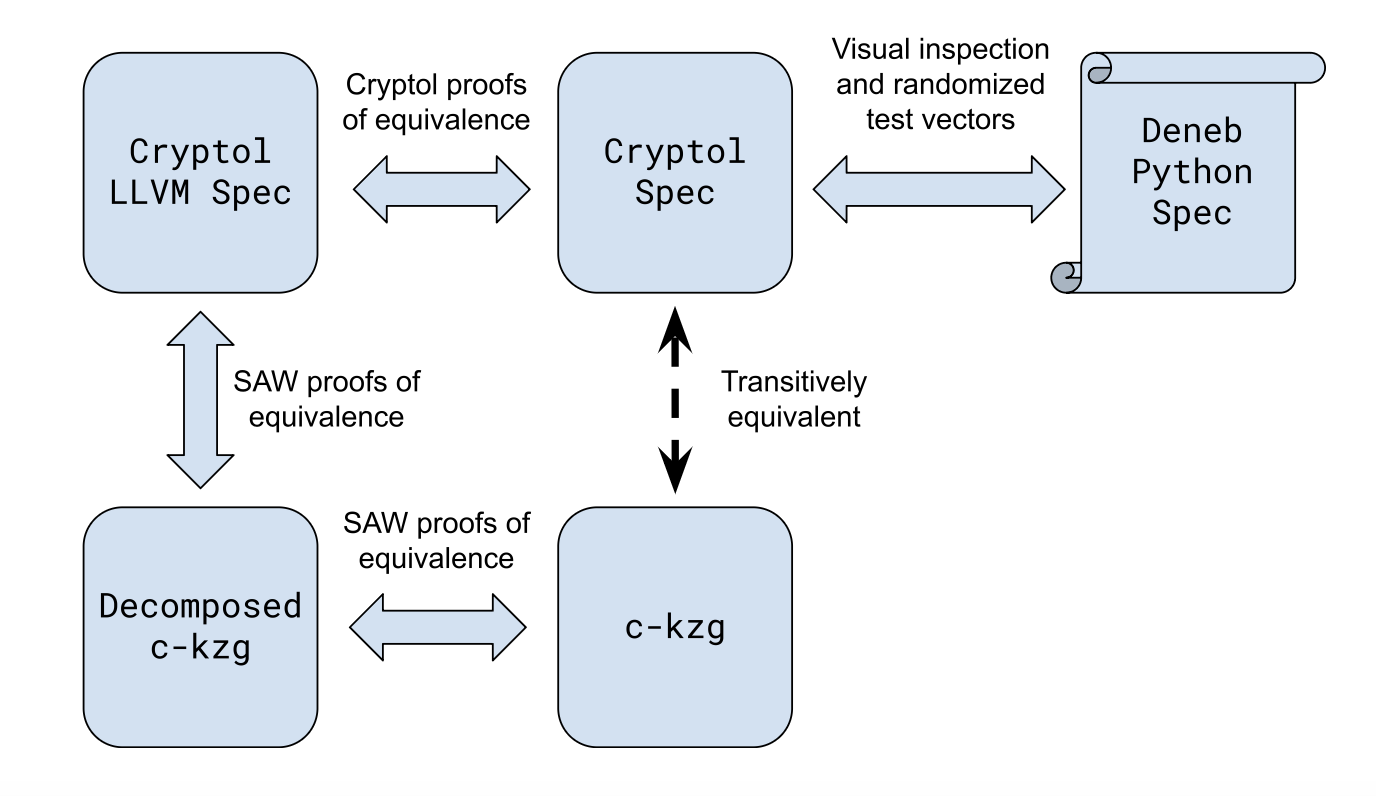
\includegraphics[width=\textwidth]{Proof-Equivalence-Diagram.png}

\section{Conclusion}

Overall, this grant was successful in funding the creation of a formal Cryptol specification of
the Python KZG Specification that can be used for further formal verification activities in both
Cryptol (which has proof language capabilities) and SAW.

The repository artifacts show a proof of concept from end-to-end for formally verifying the c-kzg
library using SAW.

\end{document}
